\subsection{Motivation}
\begin{frame} %%Eine Folie
  \frametitle{Motivation}
  
  	Tabelle mit Gegenüberstellung verschiedener Verfahren.
  	
\end{frame}
%------------------------------------------------------
\subsection{Grundlagen}
\begin{frame} %%Eine Folie
  \frametitle{Mathematische Grundlagen}
  	- Mathematische Optimierung
	- Evolutionäre verfahren
	- CMA-ES
\end{frame}
%------------------------------------------------------
\begin{frame}{Graphics} 
	\frametitle{Mathematische Grundlagen 1 }
	bla bla bla bla bla bla bla bla \\ bla bla bla bla  bla bla bla bla 
%	\begin{right} 
	\includegraphics[page=2, width=.6\textwidth]{../img/mindmap.pdf}
%	\end{right} 
\end{frame}
%------------------------------------------------------
\begin{frame}{Graphics} 
  	\frametitle{Mathematische Grundlagen }
	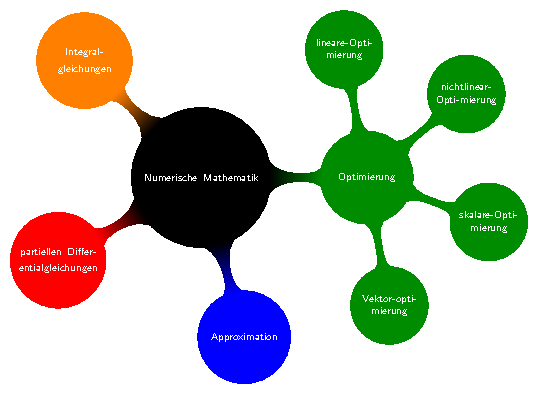
\includegraphics[page=1, width=.6\textwidth]{../img/mindmap.pdf}
\end{frame}
%------------------------------------------------------
\begin{frame}
  \frametitle{Physikalische Grundlagen}
	- Funk basierende Messung auf dem RFID-Standard 
	- Phasenmessung
\end{frame}
%------------------------------------------------------
%\subsection{Grundlagen2}
%\begin{frame}
%  \frametitle{Test}
%  \begin{fazit} %%Definition
%    Beschreibung des Problems
%  \end{fazit}
%\end{frame}
